% =====================================================================
% CHAPTER 3: Thiết kế giải thuật
% Pages 31-44 (numbered 15-28)
% Covers the 3-Tier KG-RAG algorithm design with full math derivations
% =====================================================================
\chapter{Thiết kế giải thuật}
\label{chap:thiet-ke-giai-thuat}

Chương này trình bày chi tiết kiến trúc giải thuật 3-Tier KG-RAG được đề xuất,
bao gồm phát biểu bài toán, tổng quan kiến trúc hệ thống, và ba tầng truy xuất:
duyệt cây cấu trúc hướng dẫn bởi LLM, truy xuất ngữ nghĩa hai cấp, và
Reciprocal Rank Fusion với mở rộng Knowledge Graph. Nội dung chương dựa trên
bài báo khoa học đã nộp tại hội nghị SOMET 2026 \cite{le2026threetier}.

% =====================================================================
\section{Phát biểu bài toán}
\label{sec:phat-bieu-bai-toan}

Cho tập hợp các tài liệu pháp lý được tổ chức thành một \textit{Document Forest}
(Rừng tài liệu):

\begin{equation}
  \mathcal{F} = \{T_1, T_2, \ldots, T_m\}
  \label{eq:document-forest}
\end{equation}

\noindent trong đó mỗi $T_i$ là một cây tài liệu đại diện cho một văn bản pháp lý.
Mỗi nút trong cây được gán một định danh duy nhất (node identifier) theo quy ước
phân cấp. Ví dụ, nút \texttt{59-2020-QH14:c2} ký hiệu Chương 2 của Luật
số 59/2020/QH14, còn \texttt{59-2020-QH14:d5} ký hiệu Điều 5 của văn bản đó.

Bài toán được phát biểu như sau: cho một truy vấn người dùng $q$, hệ thống cần
truy xuất $k$ điều khoản (articles) liên quan nhất từ $\mathcal{F}$, đồng thời
đảm bảo độ chính xác và khả năng giải thích kết quả.

% =====================================================================
\section{Tổng quan kiến trúc hệ thống}
\label{sec:tong-quan-kien-truc}

Hệ thống 3-Tier KG-RAG được thiết kế theo kiến trúc hai pha: pha ngoại tuyến
(offline) xây dựng các cấu trúc dữ liệu hỗ trợ, và pha trực tuyến (online)
thực hiện truy xuất theo ba tầng.

\begin{figure}[htbp]
  \centering
  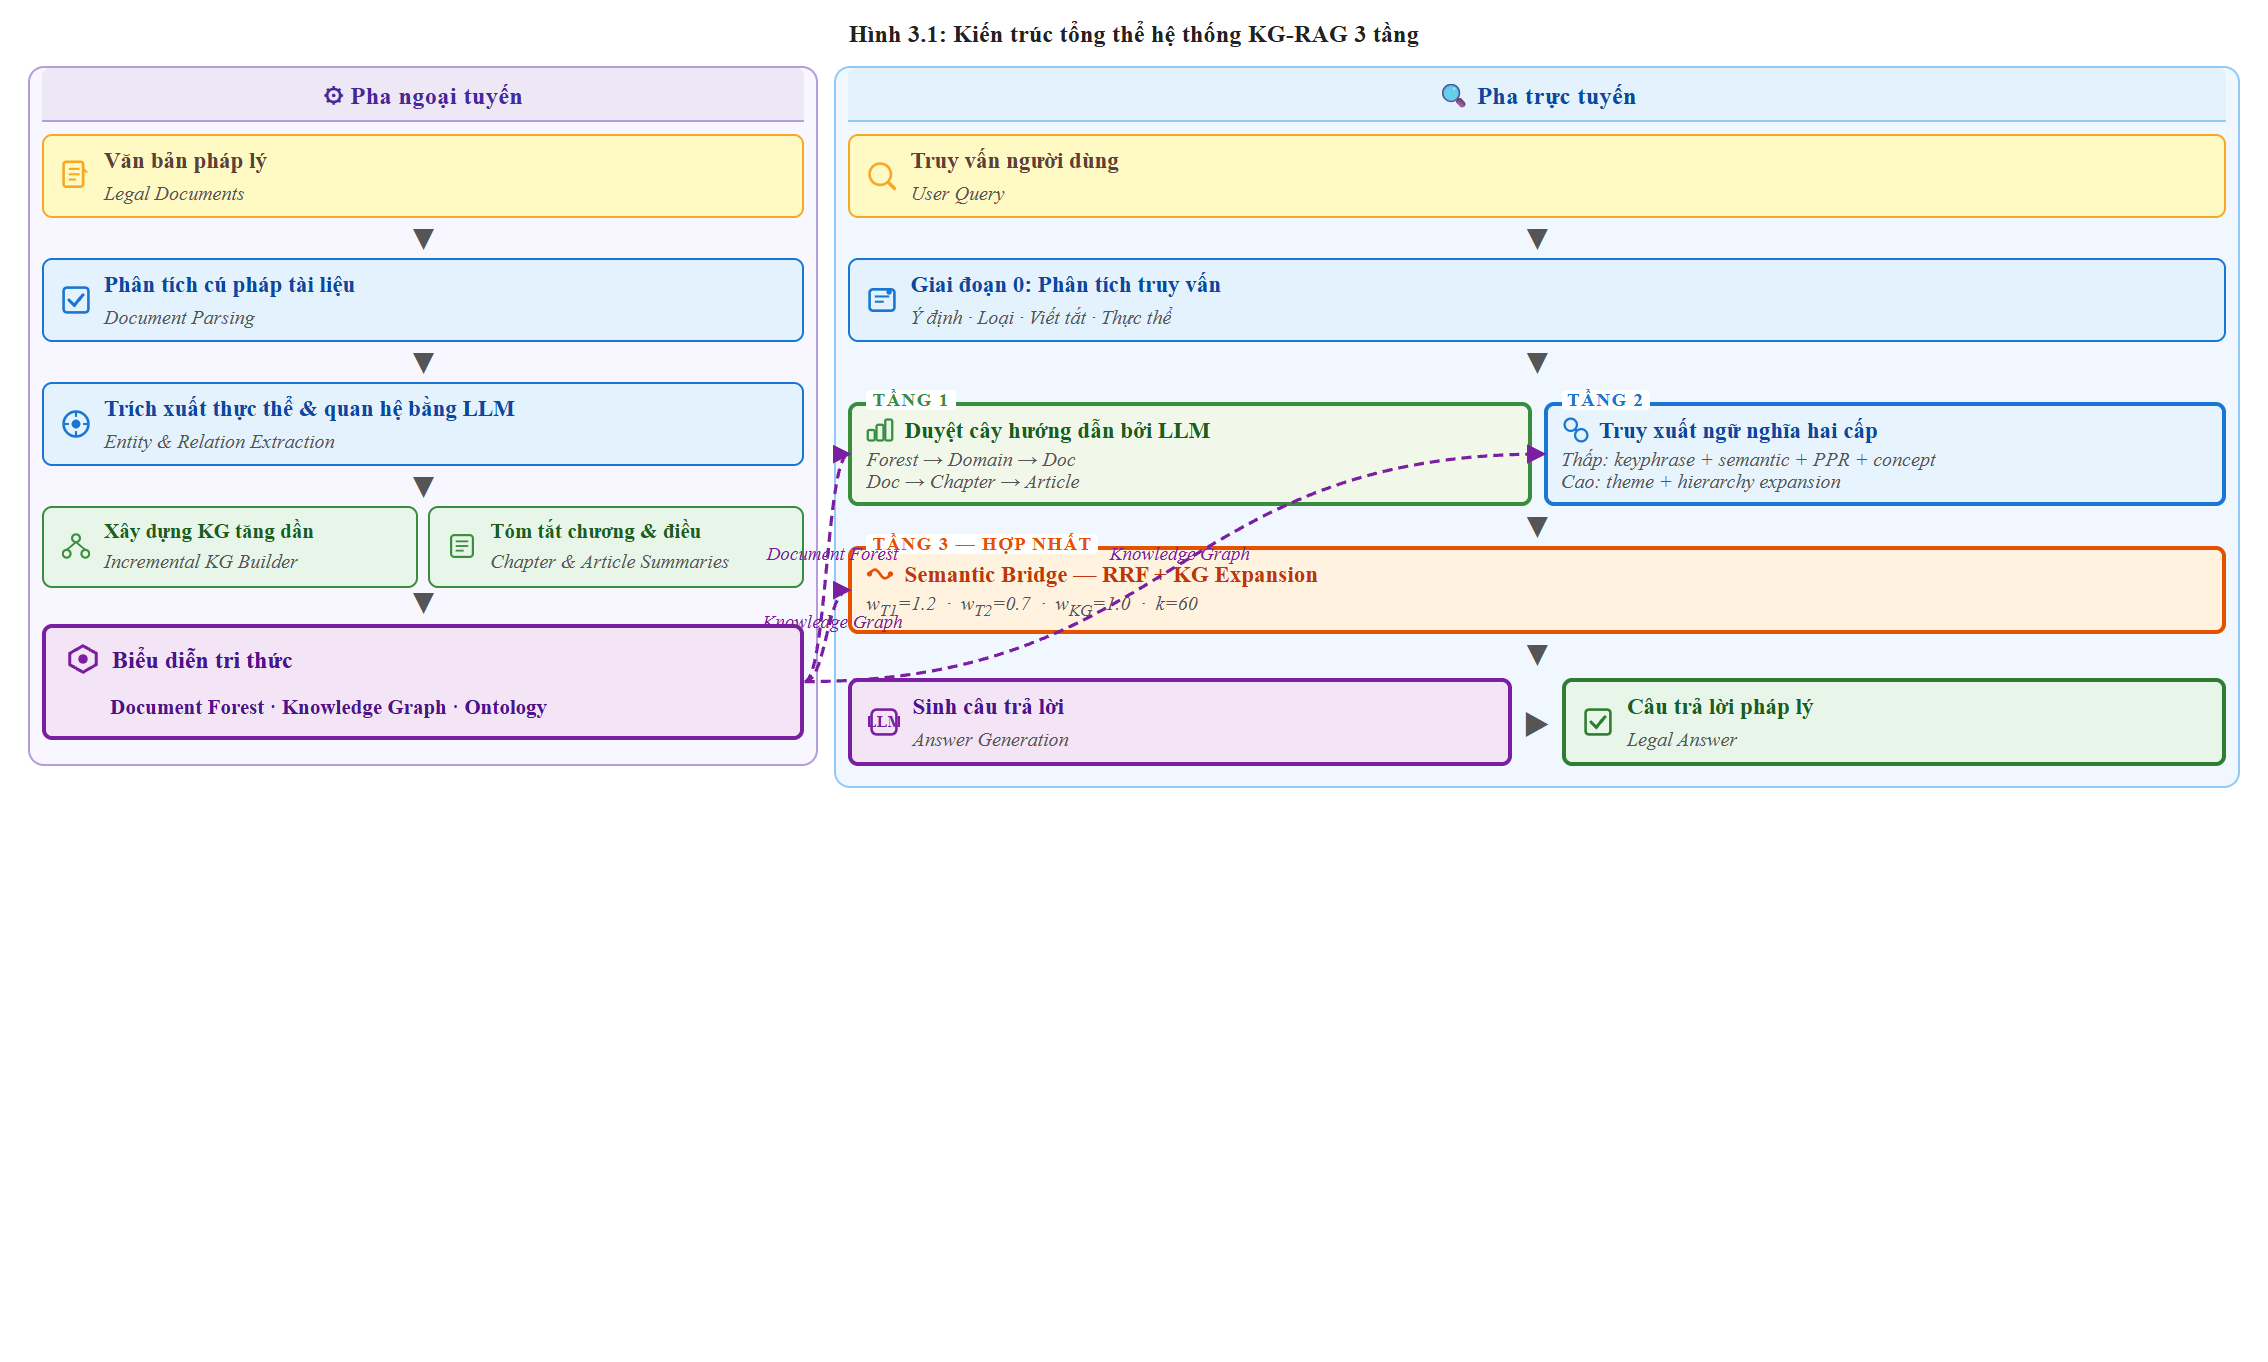
\includegraphics[width=\textwidth]{graphics/figure3-1-system-architecture.png}
  \caption{Kiến trúc hệ thống truy xuất ba tầng}
  \label{fig:kien-truc-he-thong}
\end{figure}

% -------------------------------------------------------------------
\subsection{Pha ngoại tuyến}
\label{subsec:pha-ngoai-tuyen}

\textbf{Xây dựng Document Forest.}
Mỗi tài liệu pháp lý được phân tích cú pháp và biểu diễn dưới dạng cây phân
cấp. Các nút trong cây được đặt tên theo quy tắc thống nhất mô tả trong
Bảng~\ref{tab:node-identifier-rules}.

\begin{table}[htbp]
  \centering
  \caption{Quy tắc đặt định danh nút trong Document Forest}
  \label{tab:node-identifier-rules}
  \begin{tabular}{lll}
    \toprule
    \textbf{Cấp} & \textbf{Pattern} & \textbf{Ví dụ} \\
    \midrule
    Văn bản & \texttt{\{doc\_id\}}               & \texttt{270-QĐ-ĐHCNTT} \\
    Chương  & \texttt{\{doc\_id\}:c\{N\}}         & \texttt{270:c1} \\
    Mục     & \texttt{\{doc\_id\}:s\{N\}}         & \texttt{1393:s1} \\
    Điều    & \texttt{\{doc\_id\}:d\{N\}}         & \texttt{270:d5} \\
    Khoản   & \texttt{\{doc\_id\}:d\{N\}k\{M\}}  & \texttt{270:d24k1} \\
    Điểm    & \texttt{\{doc\_id\}:d\{N\}k\{M\}p\{L\}} & \texttt{270:d24k3pa} \\
    \bottomrule
  \end{tabular}
\end{table}

\textbf{Xây dựng Summary Tree.}
Để hỗ trợ duyệt cây ở tầng 1, mỗi nút cấp văn bản, chương và mục được tóm tắt
tự động bằng mô hình Claude 3.5 Haiku. Các bản tóm tắt này cho phép LLM đánh
giá mức độ liên quan của từng nhánh cây mà không cần đọc toàn bộ nội dung.

\textbf{Xây dựng Knowledge Graph.}
Knowledge Graph (KG) được xây dựng theo quy trình bán tự động kết hợp LLM và
chuyên gia (expert-in-the-loop). Ontology sử dụng 14 loại thực thể được định
nghĩa theo chuẩn OWL với hệ thống phân cấp 4 cấp và ánh xạ nhãn tiếng Việt.
Thống kê KG được trình bày trong Bảng~\ref{tab:kg-statistics}.

\begin{table}[htbp]
  \centering
  \caption{Thống kê Knowledge Graph}
  \label{tab:kg-statistics}
  \begin{tabular}{lr}
    \toprule
    \textbf{Thành phần} & \textbf{Số lượng} \\
    \midrule
    Thực thể (entities)     & 5.936 \\
    Quan hệ (relationships) & 5.963 \\
    Loại quan hệ            & 56 \\
    Nút Document Forest     & 9.226 \\
    Tài liệu                & 13 \\
    \bottomrule
  \end{tabular}
\end{table}

% -------------------------------------------------------------------
\subsection{Pha trực tuyến}
\label{subsec:pha-truc-tuyen}

Trong pha trực tuyến, hệ thống xử lý truy vấn người dùng $q$ qua ba tầng liên
tiếp:

\begin{enumerate}
  \item \textbf{Tầng 1 -- Duyệt cây cấu trúc hướng dẫn bởi LLM:} LLM phân tích
        truy vấn và duyệt Document Forest từ gốc xuống lá, lọc ra tập ứng viên
        $C_1$ ở cấp điều.

  \item \textbf{Tầng 2 -- Truy xuất ngữ nghĩa hai cấp:} Kết hợp các tín hiệu
        ngữ nghĩa cấp thấp (keyphrase, cosine similarity, Personalized PageRank,
        concept matching) và cấp cao (theme matching, hierarchy expansion) để
        tạo tập ứng viên $C_2$.

  \item \textbf{Tầng 3 -- Hợp nhất RRF với mở rộng Knowledge Graph:} Áp dụng
        Reciprocal Rank Fusion trên $C_1$, $C_2$, và tập mở rộng từ KG để tạo
        danh sách kết quả cuối cùng.
\end{enumerate}

% =====================================================================
\section{Phân tích truy vấn}
\label{sec:phan-tich-truy-van}

Trước khi đưa truy vấn vào ba tầng truy xuất, hệ thống phân loại truy vấn thành
một trong ba loại để điều chỉnh chiến lược xử lý phù hợp:

\begin{itemize}
  \item \textbf{Keyword} (Từ khóa): Truy vấn ngắn, chứa thuật ngữ pháp lý cụ
        thể. Ví dụ: \textit{``điều kiện bảo vệ luận văn''}.

  \item \textbf{Specific} (Cụ thể): Truy vấn có ngữ cảnh rõ ràng, hỏi về một
        quy định hoặc thủ tục xác định. Ví dụ: \textit{``Học viên cần nộp hồ sơ
        gì để đăng ký bảo vệ luận văn thạc sĩ?''}.

  \item \textbf{Analytical} (Phân tích): Truy vấn mở, yêu cầu tổng hợp thông
        tin từ nhiều điều khoản hoặc so sánh quy định. Ví dụ: \textit{``So sánh
        điều kiện tốt nghiệp giữa hệ chính quy và hệ liên kết đào tạo''}.
\end{itemize}

Loại truy vấn ảnh hưởng đến trọng số của các tầng trong bước hợp nhất ở
Tầng 3 (xem Mục~\ref{sec:tang3-rrf}).

% =====================================================================
\section{Tầng 1: Duyệt cây cấu trúc hướng dẫn bởi LLM}
\label{sec:tang1-duyet-cay}

Tầng 1 sử dụng LLM để duyệt Document Forest theo chiến lược từ trên xuống
(top-down), loại bỏ sớm các nhánh không liên quan và giữ lại các ứng viên có
tiềm năng. Nhiệt độ sinh văn bản của LLM được đặt $T=0.0$ để đảm bảo tính xác
định (deterministic) trong quá trình lọc.

Quá trình duyệt cây được chia thành ba vòng lặp (loops):

\textbf{Loop 0 -- Chọn tài liệu.}
LLM nhận tóm tắt cấp văn bản của tất cả $m$ tài liệu trong $\mathcal{F}$ và
chọn ra tập con các tài liệu liên quan đến truy vấn $q$. Các tài liệu được
chọn đưa vào Loop 1.

\textbf{Loop 1 -- Chọn chương.}
Với mỗi tài liệu được chọn ở Loop 0, LLM đọc tóm tắt cấp chương và quyết định
duyệt tiếp những chương nào. Điểm ngữ nghĩa (semantic rank) được tính giữa
embedding của truy vấn và embedding của tóm tắt chương nhằm tăng cường độ chính
xác của quyết định chọn lọc.

\textbf{Loop 2 -- Chọn điều.}
Trong mỗi chương được chọn, LLM đánh giá từng điều khoản và xếp hạng chúng
theo mức độ liên quan. Ngoài điểm ngữ nghĩa đơn thuần, hệ thống áp dụng
\textit{dual rank boosting}: kết hợp cả điểm ngữ nghĩa (semantic rank) và điểm
thứ hạng kép (dual rank) để ưu tiên các điều khoản vừa liên quan về mặt ngữ
nghĩa vừa được LLM đánh giá cao.

\begin{figure}[htbp]
  \centering
  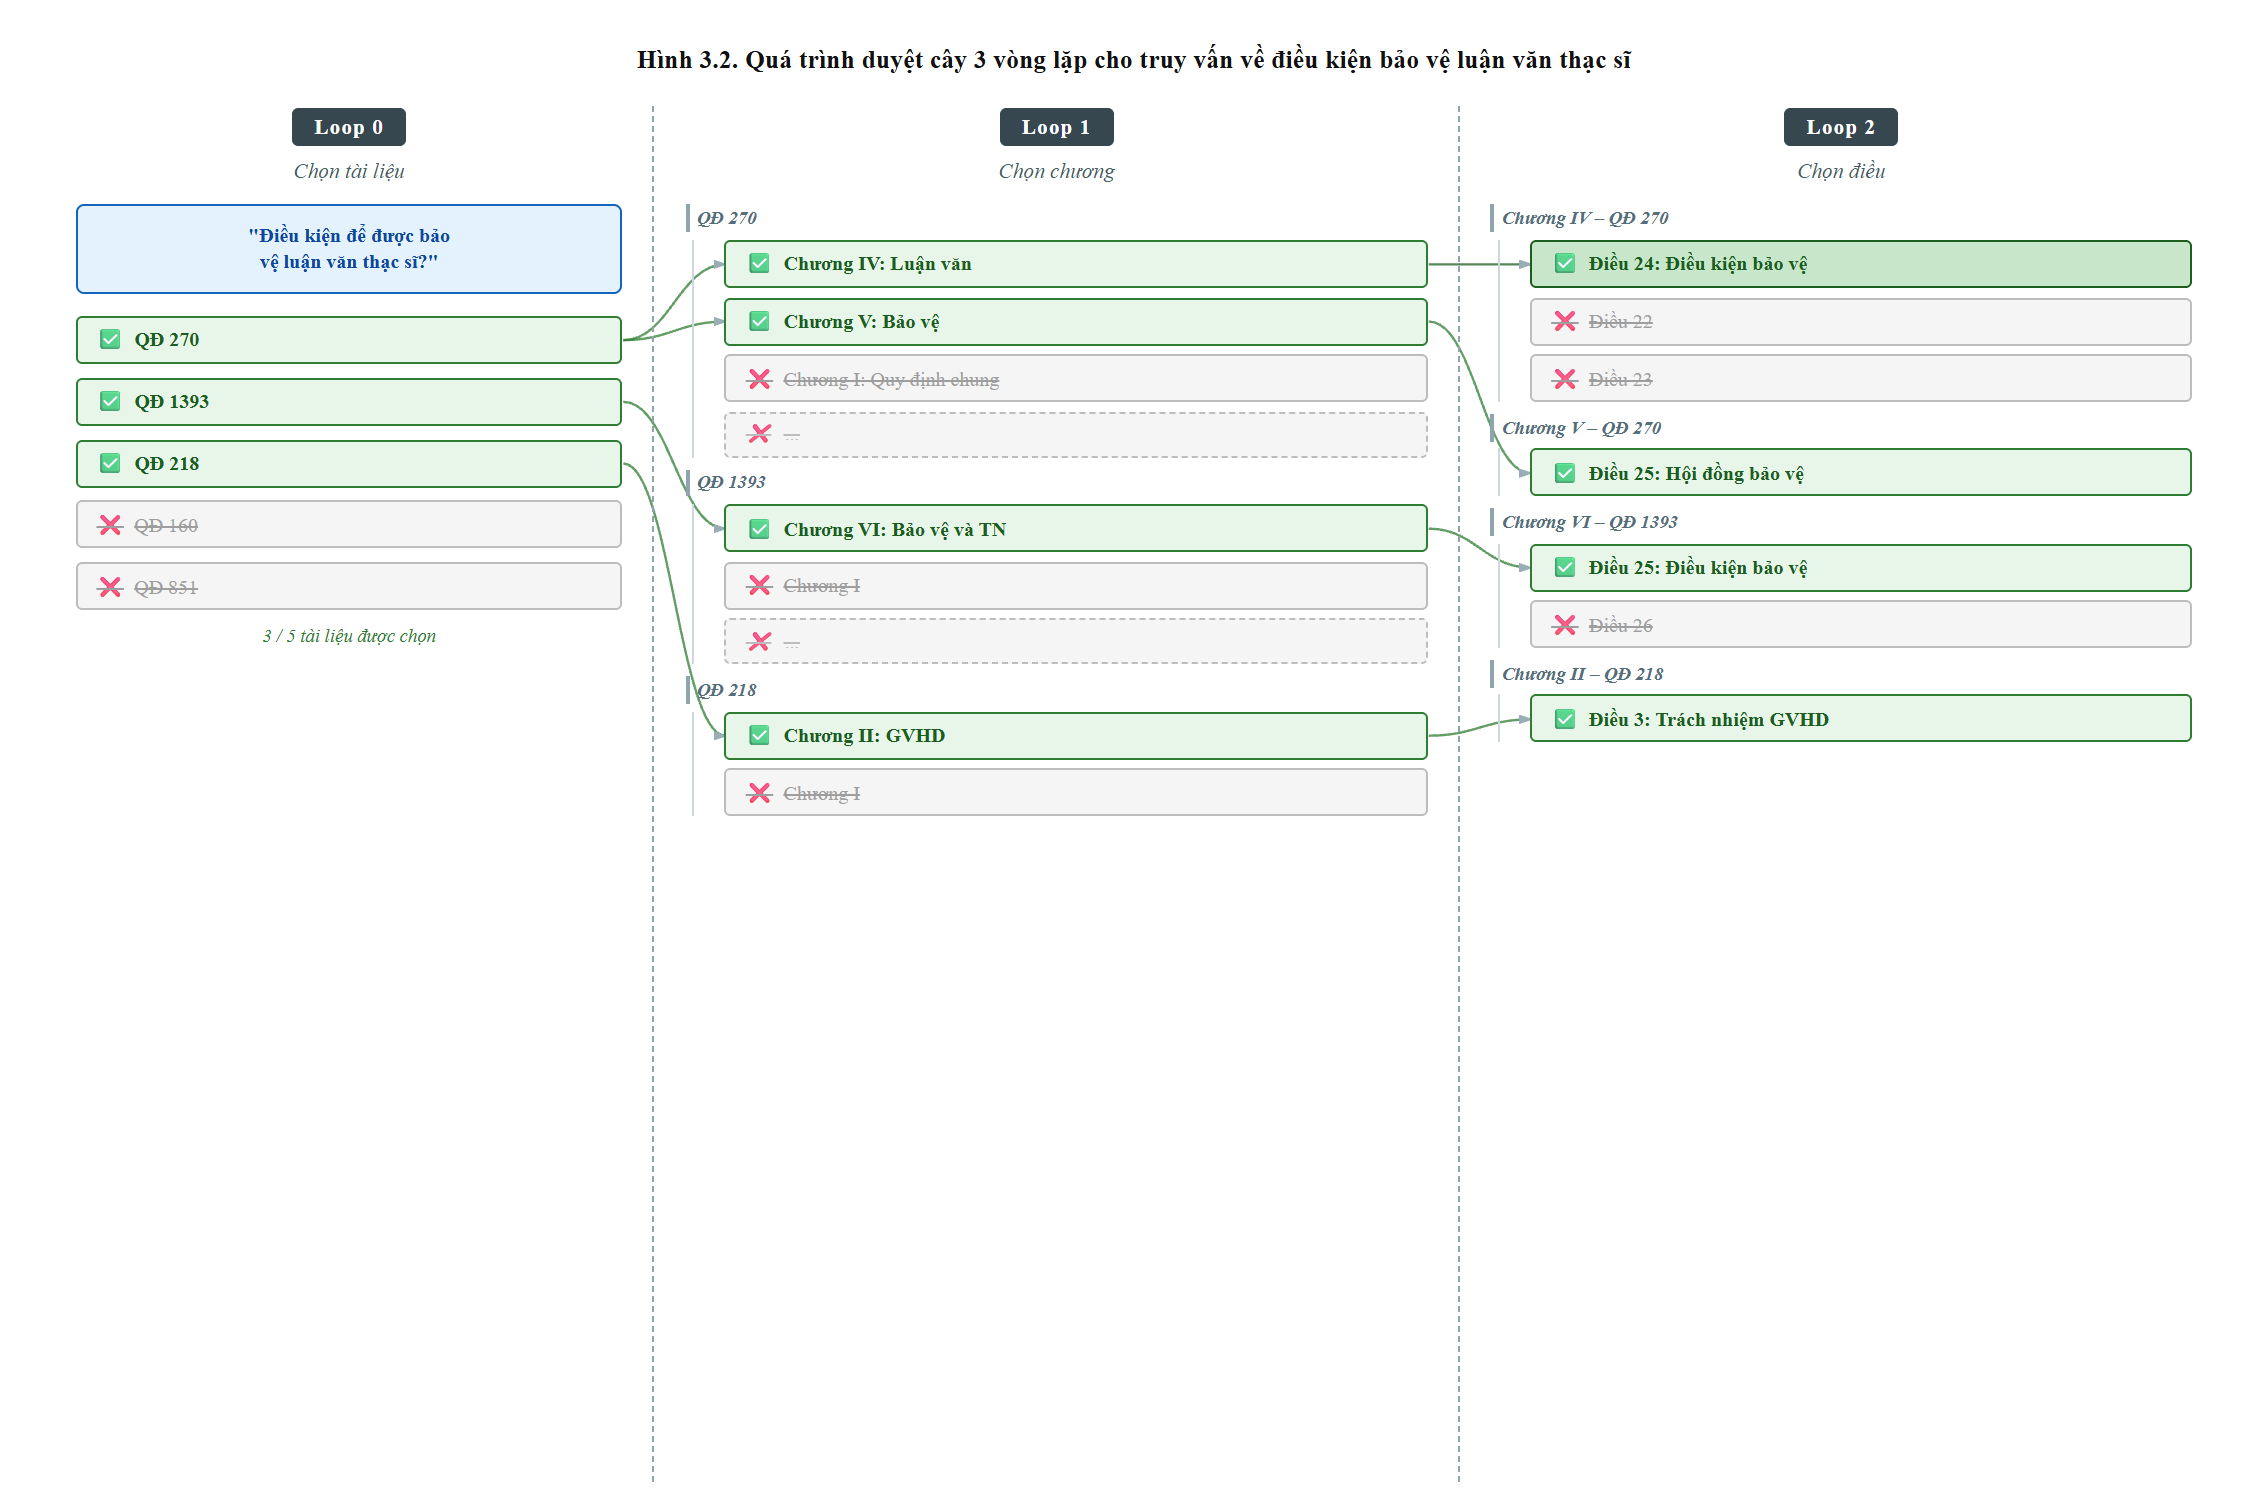
\includegraphics[width=\textwidth]{graphics/figure3-2-tree-traversal.png}
  \caption{Minh họa quá trình duyệt cây ba vòng lặp}
  \label{fig:tree-traversal}
\end{figure}

Kết quả của Tầng 1 là tập ứng viên $C_1 \subseteq \mathcal{F}$ gồm các điều
khoản được LLM xác nhận có liên quan đến truy vấn $q$.

% =====================================================================
\section{Tầng 2: Truy xuất ngữ nghĩa hai cấp}
\label{sec:tang2-semantic}

Tầng 2 tính điểm liên quan cho mỗi điều khoản ứng viên bằng cách kết hợp các
tín hiệu ngữ nghĩa ở hai cấp độ: cấp thấp (low-level, tập trung vào thực thể
và nội dung cụ thể) và cấp cao (high-level, tập trung vào chủ đề và cấu trúc
phân cấp).

% -------------------------------------------------------------------
\subsection{Truy xuất cấp thấp (Entity-specific)}
\label{subsec:low-level}

Điểm cấp thấp $s_\text{low}(a)$ cho điều khoản $a$ được tổng hợp từ bốn tín
hiệu:

\subsubsection*{1. Keyphrase Matching (Khớp cụm từ khóa)}

Hệ thống trích xuất tập thực thể $E_a$ từ điều khoản $a$ thông qua Knowledge
Graph và so khớp với các cụm từ khóa được nhận dạng từ truy vấn $q$. Điểm
keyphrase được tính như sau:

\begin{equation}
  s_\text{kp}(a) = \max_{i} (s_i) + \log(1 + n) \cdot \bar{s}
  \label{eq:keyphrase-score}
\end{equation}

\noindent trong đó $s_i$ là điểm khớp của thực thể thứ $i$ trong $E_a$, $n$ là
số lượng thực thể có điểm dương (positive entities), và $\bar{s}$ là điểm trung
bình của tất cả thực thể trong $E_a$. Thành phần logarithm $\log(1+n)$ thưởng
điểm cho các điều khoản có nhiều thực thể liên quan, thể hiện độ bao phủ chủ
đề.

\subsubsection*{2. Semantic Similarity (Tương đồng ngữ nghĩa)}

Điểm tương đồng ngữ nghĩa $s_\text{sem}(a)$ được tính bằng độ tương đồng
cosine giữa vector embedding của truy vấn $q$ và vector embedding của điều khoản
$a$, sử dụng mô hình MiniLM-L12-v2 \cite{reimers2019sbert}:

\begin{equation}
  s_\text{sem}(a) = \cos\!\left(\mathbf{e}_q,\, \mathbf{e}_a\right)
                  = \frac{\mathbf{e}_q \cdot \mathbf{e}_a}
                         {\|\mathbf{e}_q\| \cdot \|\mathbf{e}_a\|}
  \label{eq:semantic-similarity}
\end{equation}

\subsubsection*{3. Intent-aware Personalized PageRank (PPR)}

Để khai thác cấu trúc đồ thị của Knowledge Graph, hệ thống thực hiện Personalized
PageRank \cite{haveliwala2002ppr} có điều chỉnh theo ý định truy vấn. Giá trị
PPR của nút $v$ được tính theo công thức lặp:

\begin{equation}
  \text{PPR}(v) = (1-\alpha)\sum_{u \in \mathcal{N}(v)}
                  \frac{w(u,v) \cdot \text{PPR}(u)}{d(u)}
                  + \alpha \cdot p(v)
  \label{eq:ppr}
\end{equation}

\noindent trong đó:
\begin{itemize}
  \item $\alpha = 0.15$ là xác suất teleport (teleport probability),
  \item $\mathcal{N}(v)$ là tập các nút láng giềng của $v$ trong KG,
  \item $w(u,v)$ là trọng số cạnh được điều chỉnh theo ý định truy vấn
        (intent-adjusted edge weight),
  \item $d(u) = \sum_{v'} w(u,v')$ là bậc ra có trọng số (weighted out-degree)
        của nút $u$,
  \item $p(v)$ là vector cá nhân hóa (personalization vector), được thiết lập
        cao hơn tại các nút thực thể liên quan trực tiếp đến truy vấn $q$.
\end{itemize}

\subsubsection*{4. Concept Matching (Khớp khái niệm)}

Điểm khớp khái niệm đánh giá mức độ phủ của các khái niệm trọng tâm trong
điều khoản $a$ so với các khái niệm được truy vấn $q$ đề cập:

\begin{equation}
  s_\text{con}(a) = \min\!\left(1,\;
    \frac{\displaystyle\sum_{e \in E_a} w_\text{type}\!\left(\text{type}(e)\right)}
         {|E_a|}
  \right)
  \label{eq:concept-score}
\end{equation}

\noindent trong đó $w_\text{type}(\cdot)$ là trọng số gán theo loại thực thể
(entity type), phản ánh mức độ quan trọng của từng loại thực thể đối với bài
toán truy vấn pháp lý.

\subsubsection*{Tổng hợp điểm cấp thấp}

Bốn tín hiệu trên được kết hợp bằng tổng có trọng số:

\begin{equation}
  s_\text{low}(a) = w_\text{kp} \cdot s_\text{kp}(a)
                  + w_\text{sem} \cdot s_\text{sem}(a)
                  + w_\text{ppr} \cdot s_\text{ppr}(a)
                  + w_\text{con} \cdot s_\text{con}(a)
  \label{eq:low-level-combined}
\end{equation}

\noindent với các trọng số: $w_\text{kp} = 0.05$, $w_\text{sem} = 0.20$,
$w_\text{ppr} = 0.25$, $w_\text{con} = 0.20$.

% -------------------------------------------------------------------
\subsection{Truy xuất cấp cao (Conceptual)}
\label{subsec:high-level}

\subsubsection*{1. Theme Matching (Khớp chủ đề)}

Trong pha ngoại tuyến, toàn bộ các điều khoản trong $\mathcal{F}$ được phân cụm
thành các nhóm chủ đề bằng thuật toán phân cụm. Trong pha trực tuyến, truy vấn
$q$ được so khớp với top-10 cụm gần nhất theo không gian embedding. Điểm chủ đề
$s_\text{theme}(a)$ của điều khoản $a$ phản ánh mức độ gần gũi của $a$ với cụm
chủ đề phù hợp nhất với truy vấn.

\subsubsection*{2. Hierarchy Expansion (Mở rộng phân cấp)}

Điểm phân cấp $s_\text{hier}(a)$ được lan truyền từ nút cha xuống các nút con
theo hệ số suy giảm (decay factor) $\lambda = 0.5$. Cơ chế này cho phép tín
hiệu liên quan của một chương hoặc mục ảnh hưởng đến điểm số của các điều khoản
con, giảm thiểu bỏ sót do thông tin phân tán qua nhiều cấp phân cấp.

% -------------------------------------------------------------------
\subsection{Hợp nhất điểm Low-level và High-level}
\label{subsec:merge-levels}

Điểm tổng hợp cuối cùng của Tầng 2 cho điều khoản $a$ là:

\begin{equation}
  s(a) = 0.70 \cdot s_\text{low}(a)
        + 0.15 \cdot s_\text{theme}(a)
        + 0.15 \cdot s_\text{hier}(a)
  \label{eq:tier2-final-score}
\end{equation}

Các điều khoản có điểm $s(a) < 0.1$ bị loại khỏi tập ứng viên. Tập ứng viên
còn lại sau bước lọc này tạo thành $C_2$.

% =====================================================================
\section{Tầng 3: Hợp nhất RRF với mở rộng Knowledge Graph}
\label{sec:tang3-rrf}

% -------------------------------------------------------------------
\subsection{Mở rộng Knowledge Graph}
\label{subsec:kg-expansion}

Trước khi thực hiện hợp nhất, hệ thống sử dụng KG để mở rộng tập ứng viên bằng
cách bổ sung các điều khoản liên quan nhưng chưa xuất hiện trong $C_1$ hoặc
$C_2$. Quá trình mở rộng tuân theo các ràng buộc sau:

\begin{itemize}
  \item Chỉ duyệt qua các loại quan hệ \textit{mạnh} (STRONG relations):
        \texttt{references}, \texttt{requires}, \texttt{depends\_on}.

  \item \textbf{Giới hạn liên chương:} Với mỗi điều khoản nguồn, tối đa 5 điều
        khoản từ chương khác được thêm vào.

  \item \textbf{Giới hạn cùng chương:} Tối đa 2 điều khoản từ cùng chương được
        thêm vào.

  \item \textbf{Lọc ngữ nghĩa:} Chỉ giữ lại điều khoản mở rộng có độ tương đồng
        cosine với truy vấn $q$ đạt ngưỡng $\cos(\mathbf{e}_q, \mathbf{e}_a)
        \geq 0.4$.
\end{itemize}

Tập điều khoản mở rộng từ KG được ký hiệu là $C_\text{KG}$.

% -------------------------------------------------------------------
\subsection{Reciprocal Rank Fusion}
\label{subsec:rrf}

Hệ thống áp dụng Reciprocal Rank Fusion (RRF) \cite{cormack2009rrf} để hợp nhất
ba danh sách xếp hạng: $C_1$ (Tầng 1), $C_2$ (Tầng 2), và $C_\text{KG}$ (mở
rộng KG). Điểm RRF của điều khoản $d$ được tính như sau:

\begin{equation}
  \text{RRF}(d) = \sum_{s \in \{T_1,\, T_2,\, \text{KG}\}}
                  w_s \cdot \frac{1}{k + \text{rank}_s(d)}
  \label{eq:rrf}
\end{equation}

\noindent trong đó:
\begin{itemize}
  \item $k = 60$ là hằng số làm mịn (smoothing constant) theo đề xuất gốc
        \cite{cormack2009rrf},
  \item $\text{rank}_s(d)$ là thứ hạng của tài liệu $d$ trong danh sách $s$
        (bằng $+\infty$ nếu $d$ không xuất hiện trong $s$),
  \item $w_{T_1} = 1.2$, $w_{T_2} = 0.7$, $w_\text{KG} = 1.0$ là trọng số
        của từng nguồn xếp hạng.
\end{itemize}

\begin{figure}[htbp]
  \centering
  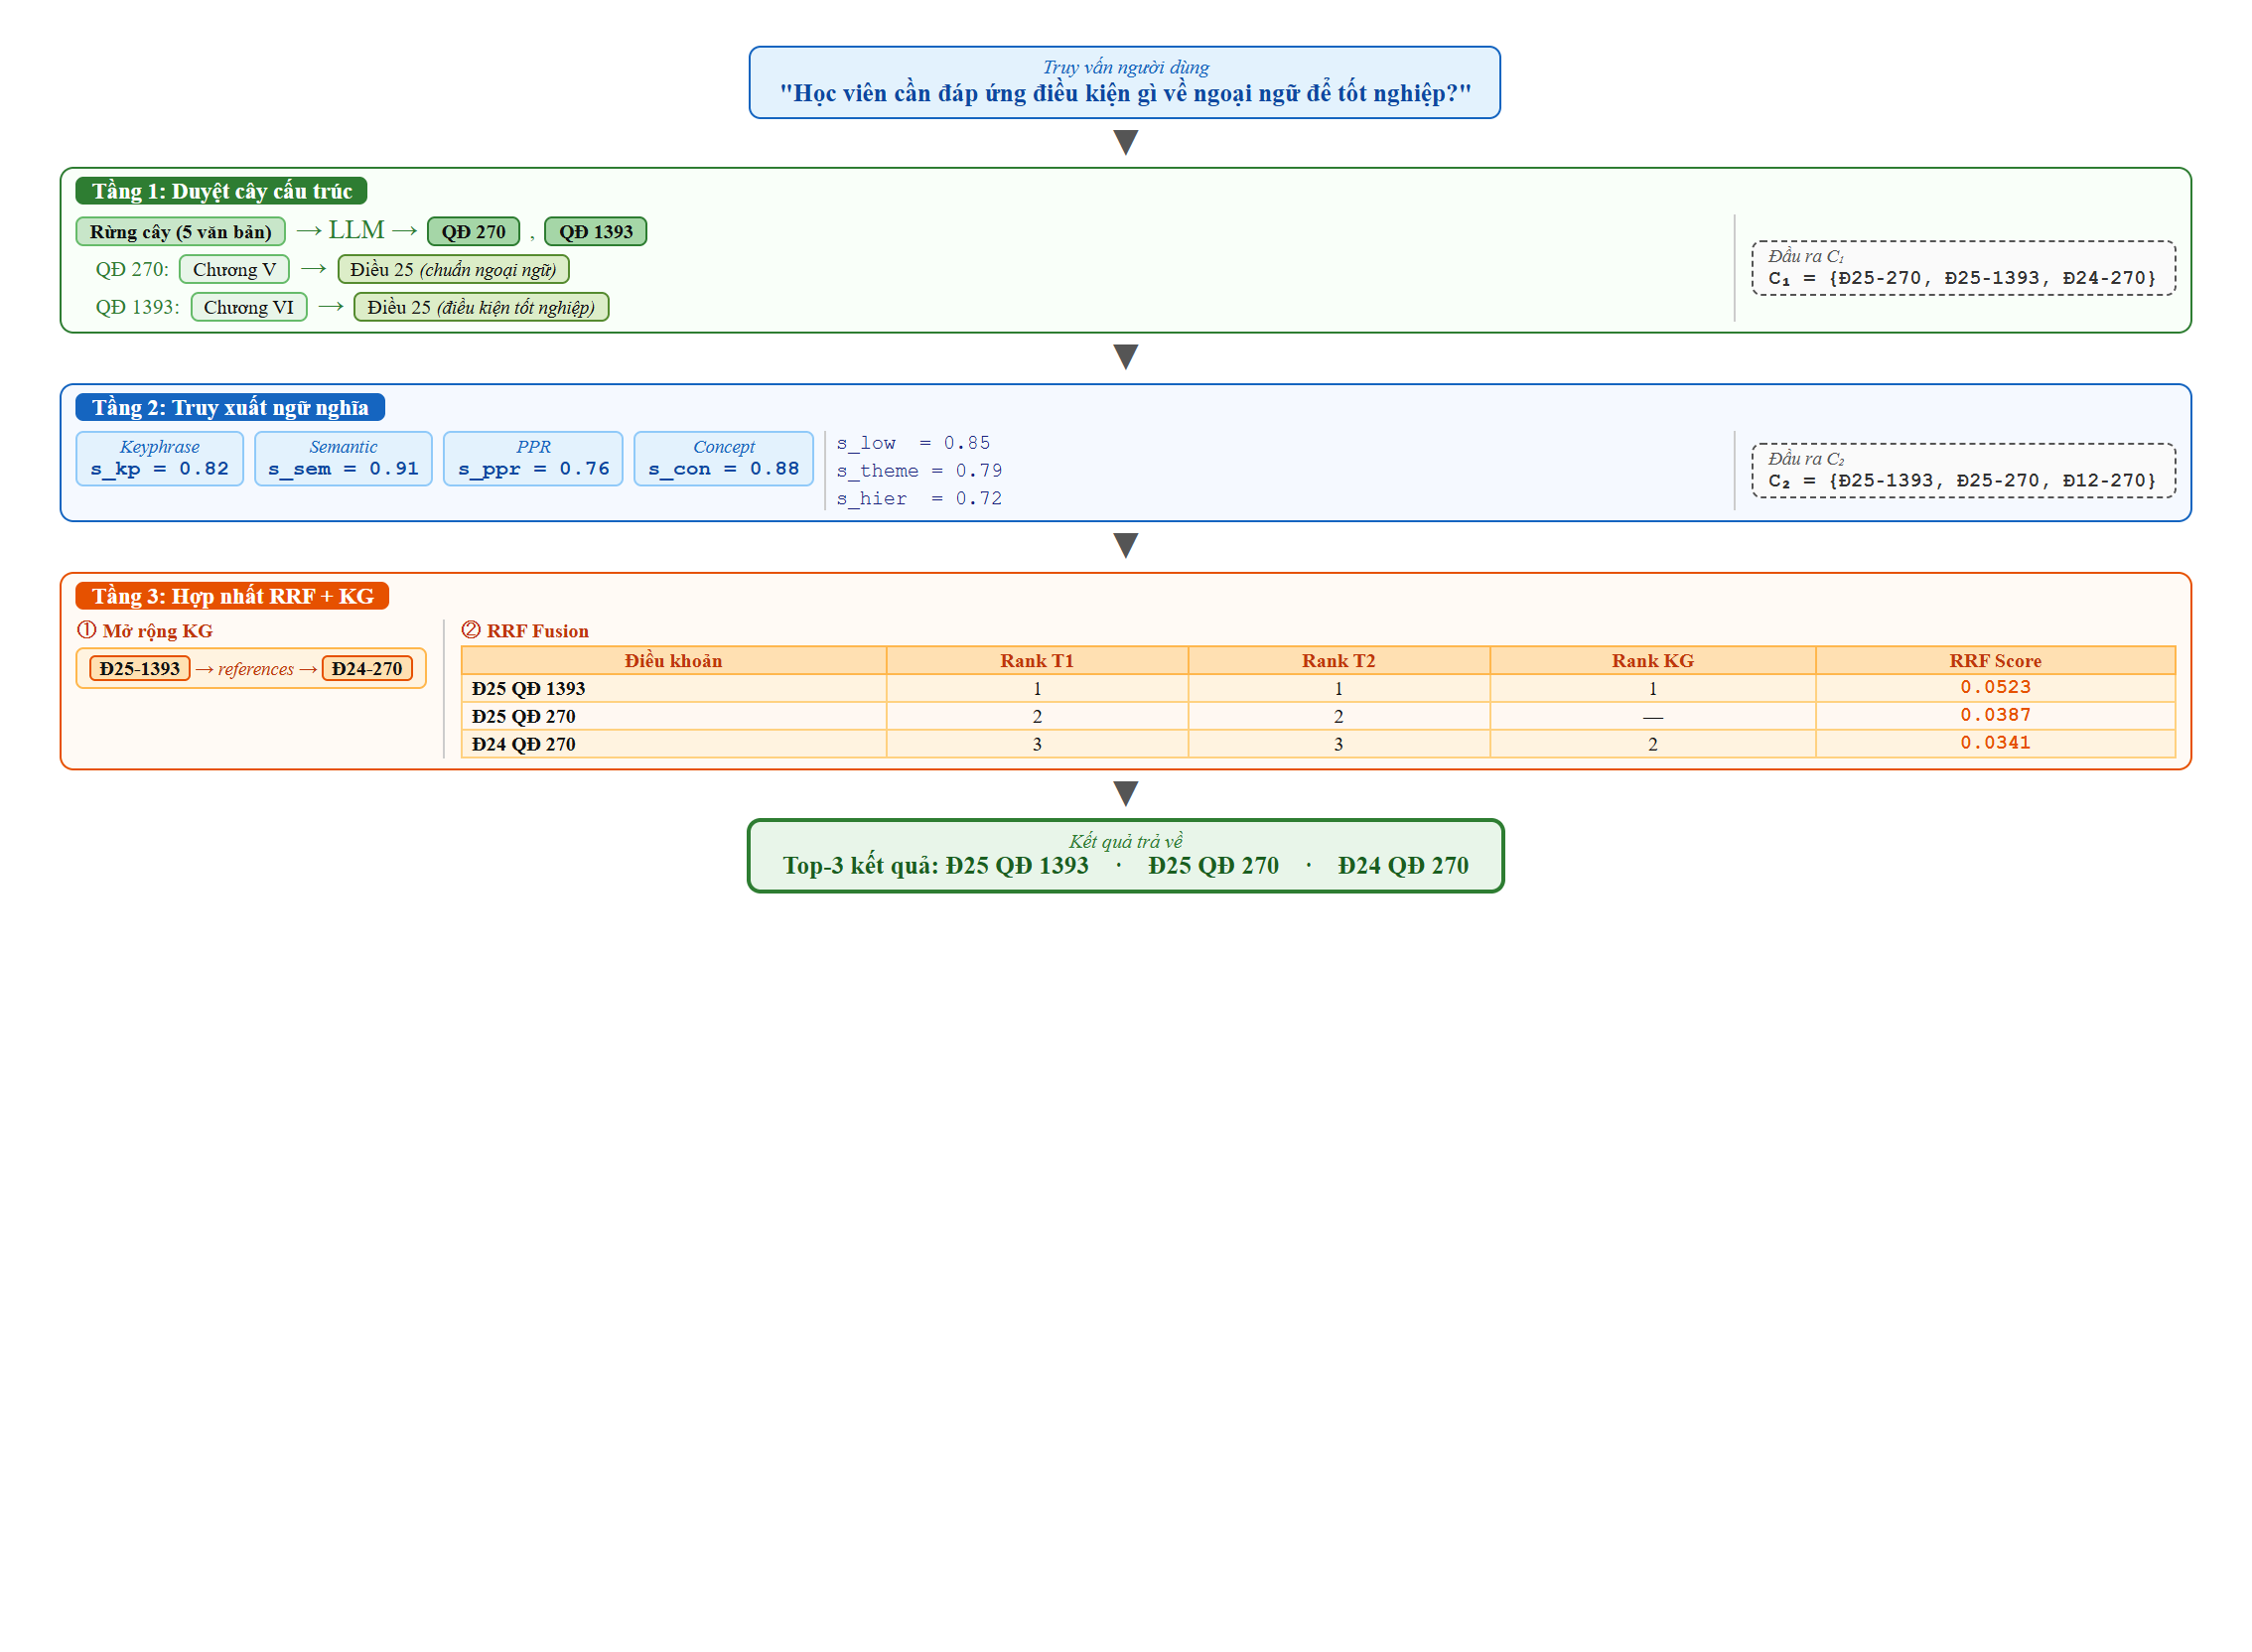
\includegraphics[width=\textwidth]{graphics/figure3-3-end-to-end-flow.png}
  \caption{Luồng xử lý end-to-end cho truy vấn điều kiện ngoại ngữ tốt nghiệp}
  \label{fig:end-to-end-flow}
\end{figure}

% -------------------------------------------------------------------
\subsection{Các cơ chế điều chỉnh}
\label{subsec:dieu-chinh}

Ngoài công thức RRF cơ bản, hệ thống áp dụng ba cơ chế điều chỉnh để nâng cao
chất lượng kết quả:

\subsubsection*{1. Dynamic Tree Weight (Trọng số cây động)}

Tầng 1 (duyệt cây) có hiệu quả thấp hơn khi truy vấn mang tính khái quát hoặc
LLM trả về phần lớn các điều khoản chung chung. Do đó, hệ thống áp dụng cơ chế
điều chỉnh trọng số động: nếu $\geq 50\%$ các điều khoản trong $C_1$ được phát
hiện là mang tính khái quát (generic), trọng số của Tầng 1 được giảm từ
$w_{T_1} = 1.2$ xuống $w_{T_1} = 0.7$, đồng thời trọng số KG được tăng từ
$w_\text{KG} = 1.0$ lên $w_\text{KG} = 1.3$.

\subsubsection*{2. Penalty (Hình phạt điểm)}

Các điều khoản thuộc các nhóm đặc biệt bị áp dụng hệ số hình phạt nhân vào điểm
RRF:

\begin{itemize}
  \item \textbf{Procedural} (Thủ tục hành chính): hệ số $\times 0.35$ — các điều
        khoản chỉ mô tả quy trình nộp hồ sơ, thời hạn hành chính, thường ít
        liên quan đến nội dung câu trả lời.
  \item \textbf{Noise} (Nhiễu): hệ số $\times 0.20$ — các điều khoản được xác
        định là không liên quan đến miền kiến thức của truy vấn.
  \item \textbf{Generic} (Khái quát): hệ số $\times 0.15$ — các điều khoản quá
        chung chung, không cung cấp thông tin cụ thể.
\end{itemize}

\subsubsection*{3. Agreement Bonus (Thưởng đồng thuận)}

Một điều khoản xuất hiện đồng thời trong nhiều tầng chứng tỏ sự đồng thuận
(agreement) từ nhiều nguồn bằng chứng độc lập, cho thấy độ tin cậy cao hơn.
Hệ thống thưởng điểm $+0.005$ cho mỗi tầng bổ sung (ngoài tầng đầu tiên) mà
điều khoản xuất hiện trong. Cụ thể, nếu một điều khoản xuất hiện trong $t \geq 2$
tầng, điểm RRF của nó được cộng thêm $(t-1) \times 0.005$.

\vspace{1em}
\noindent Danh sách kết quả cuối cùng gồm $k$ điều khoản có điểm RRF cao nhất
(sau khi áp dụng penalty và agreement bonus) được chuyển đến module sinh câu
trả lời (generation module) để tạo phản hồi cho người dùng.
